\documentclass[runningheads,envcountsame]{llncs}

\usepackage{amssymb}
\usepackage{amsmath}
\usepackage{amsfonts}

\usepackage{hyperref}
\hypersetup{
    colorlinks=true,
    linkcolor=blue,
    filecolor=magenta,      
    urlcolor=cyan
    }

\usepackage{lineno}
\usepackage{tikz}
\usepackage{graphicx}
\usepackage{thmtools}
\usepackage{thm-restate}
\usepackage{array}
\usetikzlibrary{automata, positioning, arrows}

\title{An automaton model to succinctly represent suffix-based specifications of a distributed system}

\titlerunning{An automaton model for suffix-based specifications of a distributed system}

\author{R Keerthan\inst{1,2} \and B Srivathsan\inst{2,3} \and
  R Venkatesh\inst{1}}

  \institute{Tata Consultancy Services - Innovation Labs, Pune \\
   \email{keerthanr@tcs.com, r.venky@tcs.com} \and Chennai Mathematical Institute,
  India \\
  \email{sri@cmi.ac.in} \and CNRS, ReLaX,
  IRL 2000, Siruseri, India }


  %% Macros

  \newcommand{\xra}{\xrightarrow}
  \newcommand{\Nat}{\mathbb{N}}
  \newcommand{\Aa}{\mathcal{A}}
  \newcommand{\incl}{\subseteq}
  \newcommand{\out}{\operatorname{Out}}
  \newcommand{\proj}[1]{\mathsf{P}_{#1}}
  \newcommand{\sigmain}{\Sigma_{\mathsf{In}}}
  \newcommand{\sigmaio}{\Sigma_{\mathsf{IO}}}
  \newcommand{\sigmaout}{\Sigma_{\mathsf{Out}}}
  \newcommand{\Ss}{\mathbb{TS}}
  \newcommand{\Ssf}{\Ss_{\mathsf{finite}}}
  \newcommand{\Bb}{\mathcal{B}}
  \newcommand{\Tt}{\mathcal{T}}
  \newcommand{\Ii}{\mathcal{I}}
  \newcommand{\Vv}{\mathcal{V}}
  \newcommand{\specialcell}[2][c]{%
  \begin{tabular}[#1]{@{}c@{}}#2\end{tabular}}
\newcommand{\var}{\operatorname{Var}}
\newcommand{\dom}{\ensuremath{dom}}
\newcommand{\PSPACE}{\operatorname{\textsc{Pspace}}}
  \begin{document}
  
  \maketitle

  \begin{abstract}
  Deterministic Suffix-reading Automata (DSA) were introduced recently as a
	  concise model for regular languages.  DSAs can succinctly capture formal
	  specifications that are based on \emph{sequences} of input actions (and
	  not just single actions). For a distributed system, specifications may
	  further depend on combinations of input sequences seen across multiple
	  components (ports) that communicate with each other.  For such systems, DSAs consider all possible
	  interleavings, resulting in large and unreadable automata.

  In this work, we enrich DSAs to include a $\parallel$ operator and output of letters to ports in its
	  transitions. The resulting \emph{multi-port DSAs (mDSAs)} can succinctly
	  represent concurrent suffix-based specifications. We provide a formal
	  operational semantics for mDSAs and prove that emptiness for mDSAs is
	  PSPACE-complete.  Then, we apply our results to the analysis of Expressive
	  Decision Tables (EDTs) -- an industry notation for specifying requirements
	  of reactive systems. The EDT notation has been successfully deployed in
	  various industrial settings. However, arguably, due to a complex interplay
	  between concurrency and suffix-based conditions, the notation lacks a
	  rigorous operational semantics. As a result, existing test generation
	  algorithms for EDTs do not give any theoretical guarantees. Here, we
	  provide formal operational semantics for a fragment of the EDT notation
	  using mDSAs, and reduce EDT-test-generation to mDSA-emptiness.
  
  \end{abstract}
  
  \section{Introduction}

  % Automata are very useful. In particular in formal verification and model-based testing.

  Finite state automata are all-pervasive, adopting different roles in different contexts. In this work, we focus on the role of automata as \emph{formal models of system requirements} and their subsequent application in Model Based Testing (MBT). MBT is a paradigm in formal methods where the requirements of a system under test (SUT) are first converted to a formal model. This formal model is then used to automatically generate test cases for the SUT. There are many MBT tools (see \cite{10.1145/1353673.1353681,10.1002/stvr.456} for a survey) and in several of them, the formal model is given by some extension of finite automata. 

  %Automata can be made concise.Making automata concise is a long line of work. Different ways in which they could be made concise. In MBT this helps in writing more concise specifications. 

  Converting requirements to a Deterministic Finite Automaton (DFA) or a Non-deterministic Finite Automaton (NFA) is often cumbersome. This is because DFAs and NFAs describe low level computations which reason about individual actions. There are various ways in which automata can be made consise. In Generalized Automata~\cite{DBLP:books/lib/Eilenberg76,GIAMMARRESI1999191}, transitions contain words instead of single actions. A transition $q \xra{abb} q'$ is fired from $q$ if the word $abb$ is after the automaton reaches $q$. Therefore requirements which depend on an exact sequence of actions can be represented using generalized automata more concisely. A natural extension is to allow for regular expressions in transitions, resulting in the model of Expression Automata~\cite{10.1007/978-3-540-30500-2_15} and its deterministic variant. Deterministic Expression Automata (DEA) impose restrictions on the regular expressions that can be used: they should result in a prefix-free language, and moreover, every pair of regular expressions out of state is language disjoint. This results in DEA recognizing a subset of regular languages. On the other hand, in Expression Automata, the transitions are so powerful that the states have almost no meaning: the entire automaton can be reduced to a single state and a single transition labeled by the regular expression representing the language. For languages leading to big automata, the corresponding regular expression can be complicated and incomprehensible. The goal is to hit a sweet spot where the transition labels are not too complicated, and at the same time there are fewer states than a DFA. 

   

  Deterministic suffix-reading automata (DSAs)~\cite{DBLP:journals/corr/abs-2410-22761} are a recently introduced automaton model for regular languages. Transitions are  labeled with words (as in a generalized automaton), however, the semantics is different. A transition $q \xra{abb} q'$ is fired from $q$ if a word \emph{ending} with the suffix $abb$ is seen. When there are multiple transitions out of a state, the first transition that matches is fired. Figure~\ref{fig:dsa-examples} gives some examples of DSAs.

  \begin{figure}
  \centering
  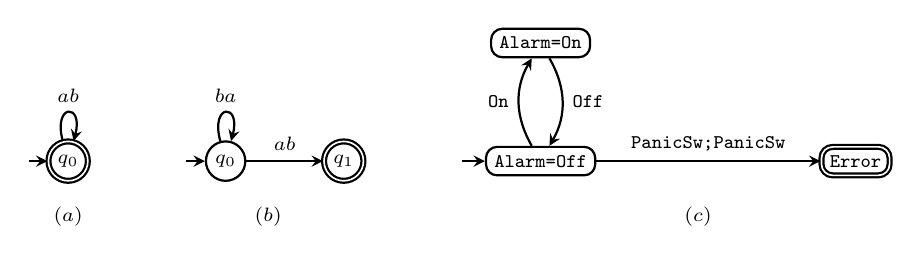
\begin{tikzpicture}[state/.style={circle, inner sep=2pt, draw, thick}]
    \begin{scope}[every node/.style={state}]
      \node [double] (0) at (0,0) {\scriptsize $q_0$};
    \end{scope}
    \begin{scope}[->, >=stealth, thick]
      \draw (-0.5, 0) to (0);
      \draw (0) to [loop above] node {\scriptsize $ab$} (0);
    \end{scope}
    \node at (0, -0.7) {\scriptsize $(a)$};

    \begin{scope}[xshift=2cm]
      \begin{scope}[every node/.style={state}]
        \node (0) at (0,0) {\scriptsize $q_0$};
        \node [double] (1) at (1.5, 0) {\scriptsize $q_1$};
      \end{scope}
      \begin{scope}[->, >=stealth, thick]
        \draw (-0.5, 0) to (0);
        \draw (0) to [loop above] node  {\scriptsize $ba$} (0);
        \draw (0) to node [above] {\scriptsize $ab$} (1);
      \end{scope}
      \node at (0.54, -0.7) {\scriptsize $(b)$};
    \end{scope}

      \begin{scope}[xshift=6cm]
        \begin{scope}
          \node [rectangle, rounded corners, draw, inner sep=3pt, thick] (0) at (0,0) {\scriptsize \texttt{Alarm=Off}};
          \node [rectangle, rounded corners, draw, inner sep=3pt, thick] (1) at (0,1.5) {\scriptsize \texttt{Alarm=On}};
          \node [rectangle, rounded corners, draw, inner sep=3pt, thick, double] (2) at (4, 0) {\scriptsize \texttt{Error}};
        \end{scope}

        \begin{scope}[->, >=stealth, thick]
          \draw (-1,0) to (0);
          \draw (0) to [bend left] node [left] {\scriptsize \texttt{On}} (1);
          \draw (1) to [bend left] node [right] {\scriptsize \texttt{Off}} (0);
          \draw (0) to node [above] {\scriptsize \texttt{PanicSw;PanicSw}} (2);
        \end{scope}
        \node at (2, -0.7) {\scriptsize $(c)$};
      \end{scope}
    
  \end{tikzpicture}
  \caption{Examples of Deterministic Suffix-reading Automata (DSA)}
  \label{fig:dsa-examples}
  \end{figure}

  In Figure~\ref{fig:dsa-examples}(a), the DSA accepts all words that end with $ab$, for instance $bab, bbab, babab$, etc. The transition $q_0 \xra{ab} q_0$ is fired as soon as a word ending with $ab$ is seen. In Figure~\ref{fig:dsa-examples}(a), we can view the state $q_0$ as tracking two suffixes $ba$ and $ab$. When $ba$ is seen before $ab$, the self-loop is triggered; otherwise when $ab$ is seen first, the transition to $q_1$ is taken. For example, on word $bbab$, the automaton starts at $q_0$, and on $bba$ it fires $q_0 \xra{ba} q_0$, reads $b$ and remains there. Since $q_0$ is non-accepting, the word is rejected. However, on $bbaab$, the run loops on $bba$ back to $q_0$, and then reads the next $ab$ to reach $q_1$, and accept. The final example Figure~\ref{fig:dsa-examples}(c) is a \emph{suffix-based specification} of a part of an automotive software: when the alarm is off, and the panic switch is pressed twice within one second, flag an error. Here, we assume there is a symbol \texttt{tick} to denote the elapse of $1$ unit of time. So, on a word \texttt{tick}; \texttt{On}; \texttt{tick} \texttt{Off}; \texttt{PanicSw}; \texttt{PanicSw}, an error should be flagged (we have added a separator symbol ; just for clarity). This specification is succinctly represented by the DSA in Figure~\ref{fig:dsa-examples}(c).

   Since transitions in a DSA wait for specific patterns to appear, DSAs are able to represent suffix-based specifications succinctly. When we consider systems with multiple components (which we call ports), the requirements can talk about different combinations of inputs. Here are two examples. 

   \begin{figure}
   \centering
   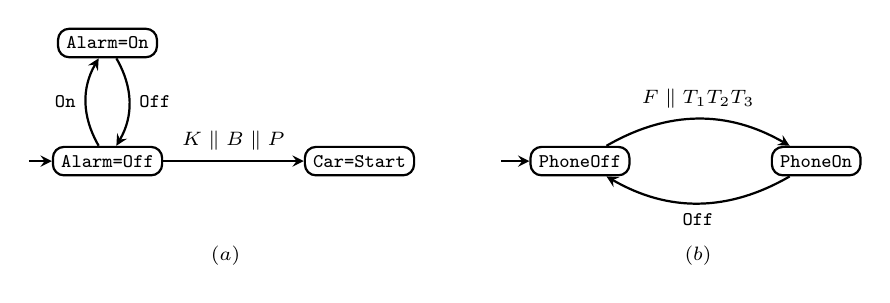
\begin{tikzpicture}
      \begin{scope}[every node/.style={rectangle, rounded corners, draw, inner sep=3pt, thick}]
        \node (0) at (0,0) {\scriptsize \texttt{Alarm=Off}};
        \node (1) at (0,1.5) {\scriptsize \texttt{Alarm=On}};
        \node (2) at (3.2,0) {\scriptsize \texttt{Car=Start}};
      \end{scope}

      \begin{scope}[->,>=stealth, thick]
        \draw (-1,0) to (0);
        \draw (0) to [bend left] node [left] {\scriptsize \texttt{On}} (1);
        \draw (1) to [bend left] node [right] {\scriptsize \texttt{Off}} (0);
        \draw (0) to node [above] {\scriptsize $K \parallel B \parallel P$} (2);
      \end{scope}

      \node at (1.5, -1.2) {\scriptsize $(a)$};

      \begin{scope}[xshift=6cm]
        \begin{scope}[every node/.style={rectangle, rounded corners, draw, inner sep=3pt, thick}]
          \node (0) at (0,0) {\scriptsize \texttt{PhoneOff}};
          \node (1) at (3,0) {\scriptsize \texttt{PhoneOn}};
        \end{scope}

        \begin{scope}[->,>=stealth, thick, auto]
          \draw (-1,0) to (0);
          \draw (0) to [bend left] node {\scriptsize $F \parallel T_1 T_2 T_3$} (1);
          \draw (1) to [bend left] node {\scriptsize \texttt{Off}} (0);
        \end{scope}

        \node at (1.5, -1.2) {\scriptsize $(b)$};


      \end{scope}
   \end{tikzpicture}
   \caption{Concurrent suffix-based specifications as multi-port DSAs}
   \label{fig:mdsa-examples}
   \end{figure}
   \paragraph*{Car Security System.} For a car to start, you need: key in ignition ($K$), brake pedal pressed ($B$), transmission in park ($P$), and no alarm triggered. The actions $K$, $B$ and $P$ can occur in any order. A DSA would need to represent this requirement using all $6$ permutations. Instead, we assume an alphabet that is distributed across different \emph{ports} -- ignition, brake pedal, transmission, and denote the concurrent actions as $K \parallel B \parallel P$. Figure~\ref{fig:mdsa-examples}(a) illustrates the enriched DSA.
  
   \paragraph*{Smartphone Lock Pattern} To unlock a phone with pattern: fingerprint verification ($F$) and drawing specific gesture with three touch points ($T_1;T_2;T_3$). This is represented as $F \parallel (T_1 T_2 T_3)$ and the enriched DSA is shown in Figure~\ref{fig:mdsa-examples}(b).
   
  In Appendix~\ref{app:examples-of-parallel}, we give many more examples of similar situations that involve multiple ports and suffix-based requirements across all of them. To the best of our knowledge, no automaton model can represent such specifications succinctly. Incorporating concurrency into the specification is paramount when requirements talk about different components of the distributed system. 
  
  \subsubsection*{Contributions.} The goal of this paper is to investigate the addition of a $\parallel$ operator into the transition syntax of DSAs. We call the resulting model as \emph{multi-port DSAs}, where the alphabet is distributed (partitioned) across multiple ports. The challenge lies in describing an operational semantics that matches with our intentions. As our first technical contribution, we provide a formal operational semantics for multi-port DSAs. 
  
  We then show that state reachability (or emptiness) for mDSAs is PSPACE-complete. For the simpler models DFAs or DSAs, reachability is linear in the input size. The higher complexity for mDSAs ties with the intuition that mDSAs can be exponentially more succinct. Our proof of PSPACE-hardness indeed exhibits such an example. 

  As our next contribution, we apply the mDSA framework to provide a formal semantics for Expressive Decision Tables (EDTs), a notation introduced by \cite{DBLP:conf/date/VenkateshSKA14} to incorporate both state-based and stream-based requirements in one convenient tabular form. The EDT notation has been successfully deployed in many industrial projects. In \cite{DBLP:conf/date/VenkateshSKA14} it has also been observed that the time and effort involved in writing EDT specifications was considerably low compared to other formalisms like  Statecharts. Many test generation tools for EDT specifications have been developed: given an EDT, and a row, the tool can generate a sequence of input actions that can trigger the input-side conditions of the particular row~\cite{DBLP:conf/enase/VenkateshSZA15a,DBLP:conf/icst/AgrawalVSZV20}. %The tricky part in the EDT notation is the use of input-output (I/O) variables that make multiple rows dependent. 
  Although EDTs have been used extensively for test generation, the notation does not yet have a formal operational semantics because of a complex interplay between concurrency and suffix-based rules. We close these gaps using the mDSA technology: we consider a fragment of the EDT notation, and map each EDT to an mDSA. This in turn gives an operational semantics for the EDT. Moreover, test generation for EDTs reduces to state reachability in mDSAs. 
  
  
  
  

  

  % Contributions. 
  % - Add a parallel operator to the syntax. Examples 2 and 3. First time that both suffix-based and concurrency have been incorporated.
  % - Challenge lies in describing an operational semantics that matches with our intentions.
  % - State reachability of mDSAs (emptiness) is PSPACE-complete. Compare with DFAs/DSAs where it is polynomial-time. This ties with the intuition that mDSAs can be exponentially more succinct.
  % - Application: EDT to mDSAs. Test generation for EDTs as emptiness of mDSAs.
  
  % Why easy-to-write specifications are important? Why formal semantics is important? 
  
  % EDT introduction. Some examples of EDTs. 

  % An intricate EDT example for which no current tool can generate a test case? 

  % Contributions

  % 2 to 3 pages

  
  \section{Related Work}
Use of automata to model distributed systems has been explored widely.
Esterel~\cite{DBLP:journals/scp/BerryG92} is a synchronous programming language
that provides a parallel composition operator. Harel's
Statecharts!\cite{DBLP:journals/scp/Harel87} also support parallel composition
of state transition systems. In both these languages the reaction of a system
in response to inputs on each port can be specified separately and the
different specifications can be composed using the parallel operator. A system
model can then refer to the states of each port's specification to model the
system behaviour. System behaviours similar to the examples described in this
paper can be specified more succinctly using mDSAs. Petri nets~\cite{CAPetri}
have been studied extensively to model concurrent systems. In Petri nets each
letter of each port's alphabet will have to be represented using a place and
the places combined to model the system. This will not be as succinct as an
mDSA. 
The work that is closest to ours is Input/Output Partial Order
Automata(IOPOA)~\cite{10.5555/2391293.2391305}. In their work transitions
execute non-atomically reacting to asynchronous inputs on several ports. The main differences between IOPOA and mDSA are - in mDSA transitions react atomically, transition labels can be strings for each port and not just letters and different transitions may trigger on the same string at a port.

  
  \newcommand{\lt}{\ell}
\newcommand{\rt}{r}

\section{Deterministic Suffix-reading Automata (DSA)}
\label{sec:prelims}

In this section, we recall the formal syntax and semantics of deterministic suffix-reading automata (DSA)~\cite{DBLP:journals/corr/abs-2410-22761}. For a finite alphabet $\Sigma$, we write $\Sigma^+$ for $\Sigma^* \setminus \{\epsilon\}$. %We provide an alternate presentation of the DSA semantics that helps extend to the mDSA model.

\begin{definition}[Deterministic Suffix-reading Automata (DSA)]
Let $\Sigma$ be a finite alphabet. A DSA $\Aa$ is given by a tuple $(Q, \Sigma, q_0, \delta, F)$ where $Q$ is a finite set of states, $q_0$ is the initial state and $F \incl Q$ is a set of final states, and $\delta \incl Q \times \Sigma^+ \times \Sigma$. Each transition therefore is of the form $(q, u, q')$ where $q, q' \in Q$ and $u \in \Sigma^*$. We write $\out(q) := \{ w \in \Sigma^+ \mid (q, u, q') \in \delta \}$.
%$\delta : Q \times \Sigma^+ \rightharpoonup Q$ is a  partial function with a finite domain. 
\end{definition}

A \emph{configuration} of a DSA is given by $(q, w)$ where $q$ is the current state, and $w$ is the word seen \emph{after reaching} $q$. The initial configuration is $(q_0, \epsilon)$. Transitions are as follows:
\begin{itemize}
\item $(q, w) \xra{a} (q, wa)$ if no string in $\out(q)$ is a suffix of $wa$,
\item $(q, w) \xra[u]{a} (q', \epsilon)$ if $u$ is the longest string of $\out(q)$ which is a suffix of $wa$, and $(q, u, q')$ is the corresponding transition. 
\end{itemize}
A configuration $(q, w)$ is accepting if $q \in F$ and $w = \epsilon$, signifying that the accepting state was reached on the last input.

 %Let $T$ be an unbounded \emph{tape} with two tape heads $\lt$ and $\rt$. We assume that the input word is written on the tape $T$, with one letter per cell. For $i \in \Nat$ we denote by $T(i)$ the letter in cell $i$ of the tape, and for $i, j \in \Nat$ with $i \le j$, we will write $T[i, j]$ for the string $T(i) T(i+1) \cdots T(j)$. Initially both the tape heads $\lt$ and $\rt$ are at position $0$, and the DSA is at its initial state $q_0$.

%Intuitively, tape head $\lt$ stores the last position when a state change happened, and $\rt$ stores the position upto which the word has been processed. Therefore, the position of $\rt$ is always to the right of $\lt$. The DSA is in some state $q$ and the tape head $\rt$ keeps moving to the right processing one letter at a time. The first instant when some string in $\out(q)$ appears as a suffix of the part of the tape between the $\lt$ and $\rt$ tape heads, a corresponding transition is triggered: DSA moves to the target state, and $\lt$ moves to $\rt$. 

%Formally, a \emph{configuration} of a DSA is given by $(q, i, j)$ where (1) $q \in Q$ is the current state of $\Aa$, (2) $i, j \in \Nat$, with $i \le j$, denote the position of the tape heads $\lt$ and $\rt$ respectively, (3) no $u \in \out(q)$ appears as a substring of the string $T[i, j]$ (which is the part of the word processed so far after the last state change). At configuration $(q, i, j)$ the DSA reads the letter $T(j+1)$.
%\begin{itemize}
%\item $(q, i, j) \xra{T(j+1)} (q, i, j+1)$ if no string of $\out(q)$ is a suffix of $T[i, j+1]$,
%\item $(q, i, j) \xra{T(j+1)} (q_u, j+1, j+1)$ if $u \in \out(q)$ is the longest string that appears as a suffix of $T[i, j+1]$ and $\Delta(q, u) = q_u$. 
%\end{itemize}
%A configuration $(q, i, j)$ is accepting if $q \in F$ and $i = j$. A \emph{run} is a sequence of transitions $\xra{}$. Notice that each word has a unique run: from a state, the first time there is a match, a transition is triggered; if there are multiple matches, we take the longest match. A word $w$ is accepted by $\Aa$ if the run of $\Aa$ on $w$ ends in an accepting configuration.

We illustrate the semantics on an example. Consider the DSA in Figure~\ref{fig:dsa-examples} (b). Here is the sequence of configurations obtained on the word $bbaab$:
\begin{align*}
(q_0, \epsilon) \xra{b} (q_0, b) \xra{b} (q_0, b) \xra[ba]{a} (q_0, \epsilon) \xra{a} (q_0, a) \xra[ab]{b} (q_1, \epsilon)
\end{align*}



  \section{Extending DSA with multiple ports}

Consider a special kind of an alphabet
$\Sigma = \langle \Sigma_1, \Sigma_2, \dots, \Sigma_k \rangle$ such
that $\Sigma_i \cap \Sigma_j = \emptyset$ for all $i, j \in
[1..k]$. We will call $\Sigma_i$ as the alphabet of \emph{port} $i$,
and $\Sigma$ as a \emph{multi-port} alphabet. We
look at DFAs over such multi-port alphabets. Such DFAs model systems
that listen to inputs from different processes and perform actions
based on them. Sometimes the order in which the system receives its
inputs from different ports is not relevant.%
  
For example, at a state
$s$, if the system receives $a$ from port 1 and $b$ from port 2, in any
order, then it has to go to state $t$.  A DFA would model this with
transitions: $s \xra{a} s_a \xra{b} t$ and $s \xra{b} s_b \xra{a}
t$. A DSA would contain two transitions $s \xra{ab, ba} t$ (and some
other transitions, if needed, to take care of $aa$, $bb$). To get a
more succinct notation we will use a $\parallel$ operator. We will
write $s \xra{a \parallel b} t$ to mean that at state $s$, when
both $a$ and $b$ are received, the automaton moves to $t$. When there
are several components, this notation leads to significant
succinctness, for instance $a_1 \parallel a_2 \cdots \parallel a_n$
stands for all the $n!$ permutations of $a_1$ to $a_n$. We will also
allow expressions of the form $a_1 a_2 \parallel b$, which stands for
the set of words $\{a_1 a_2 b, a_1 b a_2, b a_1 a_2\}$ which shuffles
$a_1a_2$ and $b$. We will now formalize this idea by enhancing DSA with
the $\parallel$ operator and then consider the problem of synthesizing
such extended DSA. We begin with some notation.%

\paragraph*{Notation.} For a word $w \in \Sigma^*$, we write
$\proj{i}(w)$ for the projection of $w$ onto the set $\Sigma_i$. For
instance, if $\Sigma_1 = \{a_1, a_2\}, \Sigma_2 = \{b_1, b_2\}$ and
$w = a_1 b_1 a_2 a_1 b_2 b_2$, we have $\proj{1}(w) = a_1 a_2 a_1$ and
$\proj{2}(w) = b_1 b_2 b_2$.  We write $\partial w$ for the $k$-tuple
$(\proj{1}(w), \proj{2}(w), \dots, \proj{k}(w))$ of projections of $w$
onto each port $\Sigma_i$, and will call $\partial w$ the
\emph{decomposition} of $w$. Notice that if
$\partial w_1 = \partial w_2$ for two words $w_1, w_2$, then $w_1$ and
$w_2$ have the same order of events within each port, but could have a
different ordering between letters from different ports.%


\paragraph*{Challenges in extending to multiport.} In a DSA, each configuration maintained the current state $q$ and the word $w$ seen after reaching $q$. This was sufficient to determine whether an outgoing transition matches. In the concurrent case, we would like our transition labels to be of the form $u_1 \parallel u_2 \parallel \cdots \parallel u_k$, with the intention that each $u_i$ is a suffix of the projection $\proj{i}(w)$. This is a natural extension so far. However, suppose a transition matches. In the DSA, we simply consume the word and go to a new configuration $(q', \epsilon)$. What is the counterpart in the concurrent case? One option is to consume the word, again, in all the ports. This is unsatisfactory: suppose the rule talks only about ports $1$ and $2$, while in state $q$ we have been receiving signals on port $3$ as well, on firing the rule, we may reach a state that depends on the signals on port $3$ received previously. Therefore, we do not want to consume the sequences seen in ports outside the fired rule. For similar reasons, sometimes we do not want to consume the letters even in the ports present in the rule. Here is an example (\textcolor{red}{TODO}). 

To cater to these different situations, we equip the automaton with multiple tape heads. Each tape head points to a position in the word seen so far. The rules can then specify the tape head since when the pattern is required to be true. Here is an example (\textcolor{red}{TODO}).

\paragraph*{Formal definition.} In multiport DSAs, the transition are labeled with a richer syntax. They make use of a parallel operator $\parallel$ and also specify a tape head.

\begin{definition} Let
  $\Sigma = \langle \Sigma_1, \Sigma_2, \dots, \Sigma_k \rangle$ be a
  multi-port alphabet. A \emph{multi-port (deterministic)
    suffix-reading automaton} (written mDSA in short) $\Aa$ is a
  tuple $(Q, \Sigma, L, q^{init}, \delta, \pi, F)$ where $Q$, $q^{init}$ and
  $F$ are a finite set of states, the initial state and a set of
  accept states, respectively; $L = \{\lt_1, \lt_2, \dots, \lt_p\}$ denotes a set of tape heads. The transition relation
  $\delta \incl Q \times (L \times\Sigma_1^* \times \Sigma_2^* \times \cdots
  \times \Sigma_k^*) \times Q$: each transition is of the form
  $(q, (\lt_j: u_1 \parallel u_2 \parallel \cdots \parallel u_k), q')$ where
  $u_i \in \Sigma_i^*$ (not all of them can be $\epsilon$) and $\lt_j$ is a tape head of $L$. We assume there are only finitely many transitions. The \emph{priority function} $\pi$ gives a total order on the set of transitions. 
 \end{definition}%

 Here is an example to illustrate the syntax of an mDSA. \textcolor{red}{(TODO)}.

 For the semantics, we assume that there is a tape on which the automaton writes all its inputs. Initially, the tape is $\epsilon$. Each time an input letter $a \in \Sigma$ is received, the automaton appends it to the right of the tape. The $p$ tape heads $\lt_1, \lt_2, \dots, \lt_p$ point to various positions in the tape. A \emph{tape configuration} is therefore given as $(T, i_1, i_2, \dots, i_p)$ where $T$ is the current word in the tape, and $i_1, \dots, i_p \in \Nat$ are the positions pointed to by the heads $\lt_1, \dots, \lt_p$ respectively. A \emph{configuration} of an mDSA is then given by a state $q$ and a tape configuration: $(q, T, i_1, \dots, i_p)$. 

Given a tape content $T$ and position $i \in \Nat$, we write $T(i)$ for the letter in the $i^{th}$ position of the tape. For two indices $i, j$ we write $T[i, j]$ to denote the substring $T(i) T(i+1) \cdots T(j)$ of the tape $T$. We will write $|T|$ to denote the length of the tape.

A transition $(q, \lt_j: u_1 \parallel u_2 \parallel \cdots \parallel u_k, q')$ matches  $(q, T, i_1, i_2 \dots, i_p)$ if
\begin{itemize}
\item $u_i$ is a suffix of $\proj{i}(T)$ for all ports $i$,
\item at least one $u_i$ occurs entirely after the tape head $\lt$: that is, $u_i$ is a subword of the word $T(i_{j}+1, |T|]$.
\end{itemize} 

Here are some examples to illustrate this definition. \textcolor{red}{(TODO)}

The formal semantics of an mDSA is given by a transition system over the configurations. The initial configuration is $(q^{init}, \vdash, 0, 0, \dots,0)$ where $\vdash$ represents a special symbol denoting the beginning of the tape (in other words, the position $0$ in the tape). All the tape heads are initially at position $0$. 
From a configuration $(q, T, i_1, \dots, i_p)$, on receiving a letter $a$, there are two possible transitions: 
\begin{itemize}
  \item $(q, T, i_1, \dots, i_p) \xra{a} (q, Ta, i_1, \dots, i_p)$, if no transition out of $q$ matches the resulting configuration $(q, Ta, i_1, \dots, i_p)$,
  \item $(q, T, i_1, \dots, i_p) \xra[\rho]{a} (q', T a, i'_1, i'_2, \dots, i'_p)$ if $\rho: (q, \lt_j: u_1 \parallel u_2 \parallel \cdots \parallel u_k)$ is the transition out of $q$ with the highest priority $\pi$, that matches $(q, Ta, i_1, \dots, i_p)$; moreover, $i'_j = |T a|$ (tape head $\lt_j$ moves to the end of the tape), and $i'_{m} = i_m$ for all other $m$ (other tape heads remain in their position).
\end{itemize}

Here are some examples to illustrate the full mechanics of an mDSA \textcolor{red}{(TODO)}.

A configuration $(q, T, i_1, \dots, i_k)$ is said to be accepting if $q \in F$ and at least one of the tape heads is in the final position $|T|$. From a technical viewpoint, this definition of accepting configurations allows us to extend DSAs. Moreover, if we think of accepting states to denote some errors, this definition ensures that as soon as a rule leading to an error is triggered, it will be accepted. \textcolor{red}{Cleaner to change to acceptance on transitions?}

\subsection{DSA is a special mDSA.}














  


  \section{Multiport DSAs with outputs}
\label{sec:multiport-outputs}

In Section~\ref{sec:multiport}, we have seen multi-port DSAs which process inputs across several ports and match transitions. In many situations, requirements also talk about outputting values to certain ports when transitions match. Here is an example of some requirements of a \emph{Car Alarm module}, adapted from~\cite{DBLP:conf/enase/VenkateshSZA15a}. 
\begin{enumerate}
\item If the most recent values on \emph{Ignition} ($I$) and \emph{Alarm} ($A$) are \texttt{Off}, and the last two values on the Panic Switch ($P$) are \texttt{Press;Press}, then the value \texttt{On} is output on the port \emph{Alarm}.

\item If the last three values on the Panic Switch are \texttt{Release;Release;Release}, and the Alarm is \texttt{On}, then output \texttt{False} on \emph{Flash} ($F$)
and \emph{Alarm}.

\item If last value on \emph{Ignition} is \texttt{On}, then \texttt{False} is output on \emph{Flash} and \texttt{Off} is output on \emph{Alarm}.
\end{enumerate}

The first requirement checks for $I:\mathtt{Off} \parallel A:\mathtt{Off} \parallel P:\mathtt{Press;Press}$ and immediately writes $A: \mathtt{On}$. The check-and-update is a fully atomic operation. One way to model this requirement as an mDSA would be to absorb port $A$ as part of the state: that is the state of the mDSA is defined using values of such ports that are used both for inputs and outputs. However, this would lead to an exponential blowup in the number of states when there are multiple such ports that are both read and written on transitions. To succinctly capture requirements with outputs, we allow both reads and writes on all ports and define \emph{mDSAs with outputs}. Later, in Section~\ref{sec:edt} we will use these mDSAs-with-outputs to give a semantics for the industry notation Expressive Decision Tables (EDTs).

\subsection{mDSA-with-outputs: formal syntax and semantics}
\label{sec:mdsao-synt}
The syntax of mDSA-with-outputs is almost the same as that of mDSAs. The only difference is in the syntax of transitions.  As before, there is a multiport alphabet $\Sigma = \langle \Sigma_1, \dots, \Sigma_k \rangle$. An mDSA-with-outputs $\Bb$ is a tuple $(Q, \Sigma, q_0, \delta)$ where $Q$ is a finite set of states, $q_0$ is the initial state and $\delta$ is a finite set of transitions. We do not view these automata as language acceptors, and so we do not specifically define accept states. We will instead discuss  state reachability. 

\paragraph*{Transitions.} A transition now looks like:
\begin{align*}
q \xra[~~O_1: b_1 ~\parallel~ O_2: b_2 ~\parallel~ \cdots ~\parallel~ O_m: b_m~~]{I_1: u_1 ~\parallel~ I_2: u_2 ~\parallel~ \cdots ~\parallel~ I_\ell: u_\ell} q'
\end{align*}
where $q, q'$ are states; each $u_j$ is a word in the port alphabet of $I_j$; and each $b_j$ is a letter in the port alphabet of $O_j$. We remark that $\{I_1, \dots, I_k\} \cap \{O_1, \dots, O_m\}$ may be non-empty. In other words, some of the ports may appear both as input and output in a transition.  

\paragraph*{Semantics.} Configurations of $\Bb$ are the same as before, given by $(q, w, \theta)$ with $q$ a state, $w$ the word seen so far and $\theta$ a position of the tape head. The semantics is a transition system $\Ss^\Bb = (S, s_0, \xra{})$ where $S$ is the set of configurations, with $s_0$ being the initial configuration $(q_0, \epsilon, 0)$. Let $\rho = (q, (I_1: u_1 \parallel \cdots I_\ell:u_\ell), (O_1: b_1 \parallel \cdots \parallel O_m: b_m), q')$. There are three kinds of transitions in $\Ss^\Bb$:
\begin{itemize}
\item \emph{$\epsilon$-transitions.} $(q, w, \theta) \xra[\rho]{~~\epsilon~~} (q', wb_1 b_2 \dots b_m, |w|)$ if the input condition ($I_1:u_1 \parallel \cdots \parallel I_\ell:u_\ell$) matches the tape configuration $(w, \theta)$; in that case move the tape head to the end of $w$ and write all the outputs to the right of $w$ (order of writing does not matter).
\item \emph{transitions on input letters.} if no outgoing transition from $q$ has a label that  matches the current tape configuration $(w, \theta)$, then there is no $\epsilon$ transition out of $(q, w, \theta)$ and the mDSA-with-outputs listens to further input letters: 
\begin{itemize}
\item $(q, w, \theta) \xra[\rho]{~~a~~} (q', wab_1 b_2 \dots b_m, |wa|)$ if $I_1:u_1 \parallel \cdots \parallel I_\ell:u_\ell$ matches $(wa, \theta)$; then, move the tape head to the end of $wa$ and write the outputs after that,
\item $(q, w, \theta) \xra{~~a~~} (q, wa, \theta)$ if no transition out of $q$ matches $(wa, \theta)$.
\end{itemize}
\end{itemize} 
Notice that the transitions on input letters have the same matching semantics as in an mDSA, except now they also write all the outputs to the end of the word. The main change is the presence of $\epsilon$-transitions. Since we write outputs after matching a transition, on reaching a new state $q'$ there could already be transitions out of $q'$ that match the current tape. Previously, in mDSA, this would not happen, since the tape head would be at the end of the word, and at least one port should see a fully fresh match. 

Surprisingly, this ability to produce outputs which can in turn be consumed by input conditions, creates complex behaviours.  We illustrate this additional difficulty by presenting an mDSA-with-outputs that can succinctly encode an $N$-bit counter.

\subsubsection*{$N$-bit counter.} We wish to implement addition of an $N$-bit counter using an mDSA-with-outputs that has $3$ states $\{q^{init}, q_0, f\}$, $N+1$ ports and $\mathcal{O}(N)$ transitions. Suppose $b_{N-1} b_{N-2} \dots b_1 b_0$ are the $N$ bits, with $b_{N-1}$ the most significant bit and $b_0$ the least significant bit. Addition can be implemented using $N$ rules: for $j \in \{0, \dots, N-1\}$
\begin{itemize}
\item if $b_j = 0$ and $b_{j-1} = b_{j-2} = \cdots = b_0 = 1$, then change $b_j:= 1$ and $b_{j-1} = b_{j-2} = \cdots = b_0 := 0$
\end{itemize}
Starting from $0$ for all bits, there will be exactly one rule that will be applicable each time. Applying the relevant rule each time will lead to $b_{N-1} = b_{N-2} = \cdots = b_0 = 1$ in $2^N - 1$ steps.

To model this counter using an mDSA-with-outputs, we can use $N$ ports $b_{N-1}, b_{N-2}, \dots, b_0$ each having two values $\{0, 1\}$. From the initial state $q^{init}$, we can first read a dummy letter (in a fresh port), write $0$ to all ports $b_{N-1}, \dots, b_0$, and move to state $q_0$. From $q_{0}$ to $q_{0}$, there is a transition for each $j \in \{0, \dots, N-1\}$ in the following form: 
\begin{align*}
q_0 \quad \xra[~~b_j:1 ~\parallel~ b_{j-1}:0 ~\parallel~ \cdots ~\parallel~ b_0: 0~~]{ b_j:0 ~\parallel~ b_{j-1}:1 ~\parallel~ \cdots ~\parallel~ b_0: 1} \quad q_0
\end{align*}
These transitions start a sequence of $2^N -1$ $\epsilon$ transitions which finally result in all ports $b_{N-1}$ to $b_0$ being $1$. To mark the end of the computation, we add an extra transition from $q_0$ that checks if $b_{N-1}:1 \parallel b_{N-1}:1 \parallel \cdots \parallel b_0:1$ and moves to $f$. Notice that the length of the tape when the automaton reaches $f$ is exponential in the size of the input automaton. Therefore, the witness for reachability is exponential. We have crucially used the ability to have ports that can be used both as inputs and outputs. We will now pin down the complexity of the reachability problem in mDSA-with-outputs. 

\subsection{Complexity of state reachability}

We now look at the state reachability problem: given an mDSA-with-outputs $\Bb$ and a state $q$, does there exist a word that reaches $q$? Without outputs, this problem is simply a graph reachability problem, like in a DFA or a DSA. The presence of outputs makes this problem harder, as seen in the $N$-bit counter.






  %\section{Complexity of emptiness}

\begin{theorem}
Emptiness for mDSA with outputs is PSPACE-complete.
\end{theorem}
\begin{proof}
    %\paragraph*{PSPACE upper bound.}
    \emph{$\PSPACE$ upper bound.} Let $\Bb$ be an mDSA-with-outputs. Consider the transition system $\Ss^\Bb$ describing the semantics of $\Bb$. Each node in the transition system is of the form $(q, w, \theta)$ where $w$ can become arbitrarily long. Therefore, the transition system, viewed as it is, is infinite. Suppose $M$ is the maximum length among all words used in the transition labels of $\Aa$. This is the maximum length of a suffix that will be checked for in a transition. To detect whether $u_1 \parallel u_2 \parallel \cdots \parallel u_k$ matches a configuration $(q, w, \theta)$, it is sufficient to maintain the last $M$ letters seen in each port. We now explain how this can be implemented.
    
    Assume that in configuration $(q, w, \theta)$, every projection $\proj{i}(w)$ of the word $w$ has at most $M$ letters. We apply the criteria for verifying if $(u_1 \parallel u_2 \parallel \cdots \parallel u_k)$ matches the tape configuration $(w, \theta)$ as in Definition~\ref{def:match}. Now, when we append $a \in \Sigma_i$ to the end of $w$: if $wa$ contains $M+1$ letters in port $i$, that is $|\proj{i}(wa)| = M+1$, then let $w'$ be the word obtained by deleting from $wa$ the first occurrence of a letter in $\Sigma_i$. Let $b$ be this letter. If $b$ appeared at a position strictly greater than $\theta$ in $wa$, then we do not need to change the tape head ($\theta' = \theta$); otherwise, $b$ appears on or before $\theta$, and we reduce tape position by $1$ ($\theta' = \theta - 1$). This gives a new tape configuration $(w', \theta')$. Call the new truncated transition system as $\Ssf^\Bb$.
    
    
    This bounds the tape length to $M \times k$, where $k$ is the total number of ports. So, the total size of the truncated transition system is exponential in the size of the input. To verify emptiness, it is sufficient to guess a path in this transition system. Since each node requires polynomial space, and the length of the witness is bounded by an exponential in the size of the input, we deduce a $\PSPACE$ upper bound for the emptiness problem, following standard results from complexity theory.

    \emph{$\PSPACE$-hardness.} For the hardness, we give a reduction from this problem: given DFAs $D_1, D_2, \dots, D_n$ over a common alphabet $\Sigma$, the DFA-intersection-emptiness asks if there exists a word in the language of all the $n$ DFAs. This is known to be $\PSPACE$-complete \textcolor{red}{Add ref}. Let $D_j = (Q_j, q^{init}_j, \delta_j, F_j)$ be the description of DFA $D_j$. The mDSA-with-outputs $\Bb^D$ that we will construct makes use of $n$ ports to store the state reached by each of the DFAs.

    We will have one input port $I$ with $\Sigma$ as alphabet, and $n$ ports $S_j$ (for $j \in \{1, \dots, n\}$), with $\Sigma_j = Q_j$ being the states of DFA $D_j$. We add a special port $L$ with alphabet $\$$ that will be used for book-keeping. Let $s^{init}$ be the initial state of $\Bb^D$. There is an initial transition that reads the special character $\$$ and writes the initial state of each DFA to the respective ports, and moves to $s_0$:
    \begin{align*}
    s^{init}~~ \xrightarrow[~S_1: q^{init}_1 ~\parallel~ S_2: q^{init}_2 ~\parallel~ \cdots ~\parallel~ S_n: q^{init}_n~]{L: \$} ~~s_0
    \end{align*}
    From $s_0$ we have a gadget that reads the next input and then sequentially updates the states of each DFA by writing the new states in the respective ports. 
    \begin{itemize}
        \item the process starts with a transition $s_0~\xra[L:\$]{I:a} s^a_1$; 
        \item there are states $s^a_{j}$ for all $j \in \{1, \dots, n\}$, and for all $a \in \Sigma$;
        \item for every transition $(q_j, a, q'_j)$ in $D_j$ we have: $s^a_j \xra[~L:\$~\parallel~S_j: q'_j~]{L:\$ ~\parallel~ S_j: q_j~} s^a_{j+1}$, with $s^a_{n+1} := s_0$.
    \end{itemize}
    When an $a$ is read at $s_0$, the automaton moves to $s^a_1$ and the tape head moves to the position of $a$. Since the same transition also writes a $\$$ to $L$, there will be an outgoing transition from $s^a_1$ that matches: this transition would be the one corresponding to the current state of $D_1$. Then, the automaton goes to $s^a_2$, and the process continues until the automaton comes back to $s_0$, giving rise to a sequence of $n$ $\epsilon$-transitions from $s^a_1$ back to $s_0$. 

    This is the basic construction that simulates the $n$ DFAs using an mDSA-with-outputs. To detect acceptance, we can add special ports $B_1, B_2, \dots, B_n$. Whenever we reach an accepting state in $Q_j$ we write $1$ to this port, and when we reach a non-accepting state, we write $1$. Add a transition $B_1 = 1 \parallel B_2 = 1 \parallel \cdots \parallel B_n = 1$ from $s_0$ to a special state $f$. The intersection of $D_1, \dots, D_n$ is empty iff $f$ is reachable.

    For every letter $a$ and every port $j$ there is a state $s^a_j$. There are transitions $s^a_j$ to $s^a_{j+1}$ for each every transition in $D_j$. Total number of states is $(|\Sigma| \cdot n) + 2$, and the total number of transitions is proportional to $\sum_j \delta_j$.  Therefore, the overall construction is polynomial-time.


\end{proof}

  

\section{Expressive decision tables}
\label{sec:edt}
Expressive Decision Tables (EDTs)~\cite{DBLP:conf/date/VenkateshSKA14} are a tabular
notation for specifying software requirements and have been used in various
industrial settings~\cite{DBLP:conf/enase/VenkateshSZA15a,DBLP:conf/icst/AgrawalVSZV20}.  An EDT specification consists
of a tables where columns specify input, output and input/output (I/O) ports, and rows specify the relationship between input and output
values on these ports. Each port is associated with an alphabet and each cell in a table consists of a string of letters from this alphabet.% with discrete
The original work on EDTs contained timing constraints in the cells and interpreted the EDT over a notion of discrete-time. In this paper we consider EDT without time. A cell in  an EDT table
is said to match when the string given in that cell is a suffix of the values seen for the
input port corresponding to that cell's column. A row of an EDT matches when
all the cells corresponding to that row match and one cell matches on the last
input.  Table~\ref{tab:edt-alarm} gives the EDT specification of the Car Alarm module described in the beginning of Section~\ref{sec:multiport-outputs}. We write $F$ for \texttt{On} and \texttt{False}, $P$ for \texttt{Press} and $R$ for \texttt{Release}. %an example, adapted from
%\cite{DBLP:conf/enase/VenkateshSZA15a,DBLP:conf/icst/AgrawalVSZV20}, specifying a subset of requirements of a car alarm
%module.

\newcolumntype{A}{>{\centering}p{1cm}}
\begin{table}[h!]
  \centering \def\arraystretch{1.5}
  \caption{EDT for an Alarm module}
  \label{tab:edt-alarm}
	\begin{tabular}{|A|A|A|A||A|c|}
    \hline
    s.no & in  I & in  P & in A & out  A & out  F \\
	 \hline
    1 & F & P;P & F& N & \\
    \hline
    2 & & R;R;R & N & F & F \\
    \hline
    3 & N & & & F & F \\
    \hline
  \end{tabular}
  
\end{table}
In the example EDT the input ports are prefixed with 
\emph{in} and output ports are prefixed with \emph{out}. Input/Output ports are prefixed with both \emph{in} and \emph{out}. These are the ports that appear on both sides of the EDT, as inputs as well as outputs. 
%The EDT of
%Table~\ref{tab:edt-alarm} specifies the
%following requirements:
%\begin{enumerate}
%	\item If the most recent values on Ports \emph{I} (Ignition) and \emph{A} (Alarm) are \emph{F}(Off), and
%		the last two values on the Port \emph{P} are $P;P$ (Press), then
%		the value \emph{N}(On) is output on the port \emph{A}.

%\item If the last three values on Port \emph{P} are
%	$R;R;R$ (Release), and the last value for \emph{A} is \emph{N}, then output the value \emph{F} (False) on \emph{F}
%		and output \emph{F} on \emph{A}.

%	\item If last value on \emph{I} is \emph{N}, then \emph{F} is output on \emph{F} 
%		and \emph{F} is output on \emph{A}.
%\end{enumerate}

A \emph{test case} for a requirement is a sequence of values  that match the
EDT row corresponding to that requirement. The use of EDTs and test case generation
algorithms from EDT specifications have been widely studied.
~\cite{DBLP:conf/enase/VenkateshSZA15a,DBLP:conf/icst/AgrawalVSZV20}. However, the notation lacks a rigorous
formal semantics, except for a brief description of key elements of formal
semantics in~\cite{DBLP:conf/date/VenkateshSKA14}. Hence, none of the test case algorithms use
formal techniques like model checking and instead rely in random generation
using heuristics. These algorithms, therefore, cannot prove that an EDT row
cannot be matched and also find it hard to match certain rows. We overcome both
these limitations by providing a formal semantics for EDTs (without timing)
through a translation to mDSA.
%When certain requirements do not get covered, a manual 
% As we will show in this paper, the mechanics of
%EDTs is intricate due to various interactions between the rows. An
%automated tool to generate test cases or \emph{guarantee}
%non-coverability is indispensable. To achieve this, the first step is
%to have a formal operational semantics for EDT.

\subsection{Translating EDT to mDSA-with-outputs}

An EDT with $I$ input columns and $R$ rows is translated to an mDSA, with one
state $q$ and an alphabet $\Sigma = \langle \Sigma_1 \cdots \Sigma_I \rangle$.
Each $\Sigma_i$ corresponds to the Port of column $i$ and the
letters of the alphabet correspond to the values that the Signal can take
prefixed by $<Portname:>$. Thus if the Port name of the first
column is $A$ and its alphabet is ${ a_1, a_2, \cdots, a_k}$ then the
corresponding alphabet $\Sigma_1 = {A:a_1, A:a_2 \cdots A:a_k}$. 
Each EDT row is translated to an mDSA as follows:
\begin{itemize}
\item The mDSA has exactly one state - $q_0$
\item 
The alphabets of all the ports together make a multi-port alphabet for the mDSA
\item
Each port has a corresponding tape. Each row has a tape head in each tape, corresponding to itself.
\item
There is a transition corresponding to each row with $q_0$ as both the source and target state. 
\item
The label of each transition consists of all the strings in the cells of the input columns of the row combined using the $||$ operator.
\item 
The output of the transitions are the strings in the cell corresponding to the output columns
\end{itemize}

The mDSA in Figure~\ref{fig:state-diagram} is a mDSA specification corresponding the EDT given in Table~\ref{tab:edt-alarm}

\begin{figure}[htbp]
    \centering
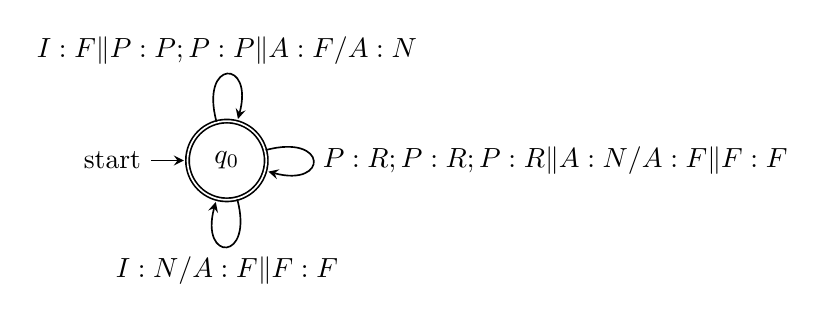
\begin{tikzpicture}[
    > = stealth,
    shorten > = 1pt,
    auto,
    node distance = 3cm,
    semithick
]

% Setup the styles for the states
\tikzstyle{accepting}=[double, draw=black, circle, minimum size=1cm]
\tikzstyle{state}=[draw=black, circle, minimum size=1cm]

% Draw the state
\node[state, initial, accepting] (q0) {$q_0$};

% Draw the transition (self-loop)
\draw (q0) edge[loop above] node{$I:F$$\|$$P:P;P:P$$\|$$A:F$/$A:N$} (q0);
\draw (q0) edge[loop right] node{$P:R;P:R;P:R$$\|$$A:N$/$A:F$$\|$$F:F$} (q0);
\draw (q0) edge[loop below] node{$I:N$/$A:F$$\|$$F:F$} (q0);

\end{tikzpicture}
\caption{mDSA of the Alarm EDT}
    \label{fig:state-diagram}
\end{figure}


%%The mDSA above is a succinct representation of the EDT semantics. The states of a multi-port DSA are defined as per the requirements of the system it models. For a system with internal variables $S_1,S_2,\dots$ with each variable $S_i$ having an alphabet $\Sigma_{S_i}$, the corresponding \mdsa has states $Q=\Sigma_{S_1} \times \Sigma_{S_2} \times \dots$, but as seen earlier, this can be captured using additional tape instead. The additional tapes $B_{S_1}, B_{S_2}, \dots$ are for the internal variables used in the system. These variables can read input as well as produce output, over the alphabet representing their state space. %For example, a variable $S_i$ has an alphabet $\Sigma_{S_i}$ with letters that can be input as well as output.
%%
%%Transitions must then be enhanced in our semantics i.e. a transition can now require the local variables $S_1, S_2,\dots$ to have values $(s_1, s_2 \dots)$  for it to match. When triggered, the values then change to $(s'_1,s'_2,\dots)$. Assume each variable $S_i$ has its corresponding tape labeled $B_{S_i}$%(we relabel the tapes $B_{k+1}, B_{k+2}, \dots, B_{k'}$ appropriately)
%%. Let us use the syntax $\langle (s_1, s_2 \dots), (u_1, \dots, u_k), (s'_1,s'_2,\dots) \rangle$ to represent this.
%%
%%\begin{enumerate}
%%\item A transition (with label $j$) $\langle (s_1, s_2 \dots), (u_1, \dots, u_k), (s'_1,s'_2,\dots) \rangle$ is matched if each $B_i (i\le k)$ has $u_i$ as suffix, the last letter of each $B_{S_i}$ is $s_i$, and either $H_{i}^{j}$ is at the end or the entire $u_i$ is after $H_{i}^{j}$. Additionally, at least one tape is non-empty after $H_{i}^{j}$.
%%
%%\item A matched transition is then triggered, moving each $H_{i}^{j}$-head of $B_i$ (or $B_{S_i}$) to the end. Additionally $\forall s'_i \ne \epsilon$, the corresponding $B_{S_i}$ extends by one position to the right and stores $s'_i$.
%%\end{enumerate}
%%
%%\textcolor{red}{Semantics for Row sequences}
%%We introduce the notion of a multi-transition, a transition with multiple parts that must occur in sequence. Let us illustrate with a two-part transition $\langle (s_1, s_2 \dots), (u_1, \dots, u_k), (s'_1,s'_2,\dots)$ ; $(s''_1, s''_2 \dots), (u'_1, \dots, u'_k), (s'''_1,s'''_2,\dots) \rangle$. For it to match, each $B_i (i\le k)$ must have $u_i  u'_i$ as suffix, each $B_{S_i}$ has $s_i  s''_i$, and either $H_{i}^{j}$ is at the end or the entire $u'_i$ occurs after $H_i^j$. Additionally, at least one tape is non-empty after $H_i^j$ heads. Not only this, all of $(s''_1, s''_2 \dots), (u'_1, \dots, u'_k)$ must occur after $(s_1, s_2 \dots), (u_1, \dots, u_k)$. That is each for any $i,j$ we have $u'_i$ and $s''_i$ appearing after $u_j$ and $s_j$. When the matched transition is triggered, the tapes and their head positions are updated as earlier.
%%
%%\textcolor{red}{TODO: Reachability for mDSA vs Test generation for EDT. Complexity result (possibly PSPACE-complete)}
%%
%\input{basic.tex}


%%% Local Variables:
%%% mode: latex
%%% TeX-master: "mDSA"
%%% End:


  %\section{Experiments and Conclusion}

  \section{Experiments}
\label{sec:experiments}
A testsuite $\Pi(\Tt)$ for an EDT $\Tt$ is a set of executions such
that for each row $R$ of $\Tt$ there exists an execution
$\pi \in \Pi$ and $\pi$ triggers $R$. To find a testsuite, we need to solve the test generation problem for each row.
%The testsuite generation problem is to check whether there exists a testsuite for a given EDT.

We have developed a prototype tool that implements an
algorithm to solve the test generation problem by systematically
exploring the configurations of an mDSA corresponding to the given EDT,
$\Tt$.  %The tool does not handle timing.

We conducted experiments to validate the following:

\begin{enumerate}
\item For simple EDTs, the tool can find test cases succesfully.
\item There are some EDTs for which it can solve the test
  generation problem, where randomized techniques (likely) cannot.
\end{enumerate}

%\texttt{Random} uniformly samples a set of executions, $\Pi_R(\Tt)$, of size
%$N$, from the universal set of executions that have exactly $P$ inputs
%and checks whether $\Pi_R(\Tt)$ is a testsuite for $\Tt$. \texttt{RGRaF}, on
%the other hand, employs a heuristic to sample a set of executions of
%size $N$ and checks whether it is a testsuite. \texttt{RGRaF} takes a parameter
%$P$ to restrict the number of inputs in each execution.

First we look at a couple of small EDTs. Table~\ref{tab:alarm-2} gives an example motivated from
\cite{Venkatesh:ENASE:2015} which describes selected requirements of a
car alarm module. It is similar to Table~\ref{tab:edt-alarm} from Section~\ref{sec:edt}. Encoding this in our tool gives a testcase (Press; Press) for Row 1.

\begin{table}[h!]
  \centering \def\arraystretch{1.2}
  \caption{EDT for an Alarm module}
  \label{tab:alarm-2}
  \begin{tabular}{|c|c|c|c||c|c|}
    \hline
    sno & \specialcell{in \\ Ignition} &
                                         \specialcell{in \\ PanicSw} &
                                                                       \specialcell{in 
    \\ Alarm} & \specialcell{out \\ Alarm} & 
                                             \specialcell{out \\ Flash} \\
    \hline 
    1 & Off & (Press; Press)%\{$<1$s\} 
    & Off & On &
    \\
    \hline

    2 & On & & & Off & False \\
    \hline
  \end{tabular}
  
\end{table}

Next we look at Table~\ref{tab:wiper}, a partial representation of a wiper module in a car. The tool finds a testcase for Row 2.

\begin{table}[h!]
  \centering \def\arraystretch{1.2}
  \caption{EDT for a Wiper module}
  \label{tab:wiper}
  \begin{tabular}{|c|c|c|c|c||c|c|}
    \hline
    sno & \specialcell{in \\ ignition} &
                                         \specialcell{in \\ wiperswitch} & 
                                                                       \specialcell{in 
    \\ parksensor} & \specialcell{in \\ error} & \specialcell{out \\ wipercmd} & 
                                             \specialcell{out \\ error} \\
    \hline 
    1 & on & on & 
    & false & wipe &
    \\
    \hline

    2 & & & (park;notpark) & & dontwipe & true \\
    \hline
  \end{tabular}
  
\end{table}


For the other claim, we created a specific kind of EDT for
which the probability of randomized techniques selecting a required
execution is very low. The EDT extends the three bit counter,
shown in Table \ref{tab:binary}, to five bits and adds a 
row to reset the counter. Our tool solves this problem, and hence for rows that have a very low probability of getting triggered
it is better than randomized techniques.

%Table \ref{tab:binary} shows a counter for $3$ bits.

\begin{table}
  \centering
  \renewcommand{\arraystretch}{1.2} 
  \caption{Implementing a binary counter for $3$ bits}
  \label{tab:binary}
  \begin{tabular}{|c|c|c|c|c||c|c|c|c|}
    \hline
    $T$ & $t_2$ & $t_1$ &$t_0$ & $S_T$ & $t_2$ & $t_1$ & $t_0$ & $S_T$                                                             
    \\
    \hline
     \checkmark & & & & & & & & $+$  \\
         
    \hline
     & & & $0$ & $+$ & & & $1$ & $-$  \\

    \hline
   & & $0$ & $1$ & $+$ & & $1$ & $0$ & $-$ \\

    \hline
   & $0$ & $1$ & $1$ & $+$ & $1$ & $0$ & $0$ & $-$ \\

    \hline
  \end{tabular}
\end{table}


%%% Local Variables:
%%% mode: latex
%%% TeX-master: "m"
%%% End:


  \section{Related Work}
Use of automata to model distributed systems has been explored widely.
Esterel~\cite{DBLP:journals/scp/BerryG92} is a synchronous programming language
that provides a parallel composition operator. Harel's
Statecharts!\cite{DBLP:journals/scp/Harel87} also support parallel composition
of state transition systems. In both these languages the reaction of a system
in response to inputs on each port can be specified separately and the
different specifications can be composed using the parallel operator. A system
model can then refer to the states of each port's specification to model the
system behaviour. System behaviours similar to the examples described in this
paper can be specified more succinctly using mDSAs. Petri nets~\cite{CAPetri}
have been studied extensively to model concurrent systems. In Petri nets each
letter of each port's alphabet will have to be represented using a place and
the places combined to model the system. This will not be as succinct as an
mDSA. 
The work that is closest to ours is Input/Output Partial Order
Automata(IOPOA)~\cite{10.5555/2391293.2391305}. In their work transitions
execute non-atomically reacting to asynchronous inputs on several ports. The main differences between IOPOA and mDSA are - in mDSA transitions react atomically, transition labels can be strings for each port and not just letters and different transitions may trigger on the same string at a port.


  \bibliographystyle{plain}
  \bibliography{mDSA-netys.bib}

  \appendix

  
\section*{Parallel Operator Examples}

The parallel operator ($\|$) is indeed useful for showing that two conditions must both be satisfied but the order doesn't matter. Here are some examples where the parallel operator becomes increasingly advantageous with more inputs:

\subsection*{Car Security System}
For a car to start, you need: key in ignition ($K$), brake pedal pressed ($B$), transmission in park ($P$), and no alarm triggered ($A$).
\begin{itemize}
    \item Sequential: $K;B;P;A$ or any of the 24 possible permutations
    \item Parallel: $K\|B\|P\|A$ (much more compact)
\end{itemize}

\subsection*{Home Theater Setup}
To watch a movie, you need: TV on ($T$), sound system on ($S$), streaming device connected ($D$), internet working ($I$), and appropriate app opened ($A$).
\begin{itemize}
    \item Sequential: $T;S;D;I;A$ or any of the 120 possible permutations
    \item Parallel: $T\|S\|D\|I\|A$
\end{itemize}

\subsection*{Computer Boot Sequence}
For proper boot, you need: power supply working ($P$), motherboard operational ($M$), CPU functioning ($C$), RAM installed ($R$), storage device connected ($S$), and BIOS loaded ($B$).
\begin{itemize}
    \item Sequential: Would require one of 720 possible orderings
    \item Parallel: $P\|M\|C\|R\|S\|B$
\end{itemize}

\subsection*{Chemical Reaction Prerequisites}
For a particular reaction to occur, you need: correct temperature ($T$), proper pressure ($P$), catalyst present ($C$), reagent A ($A$), reagent B ($B$), and appropriate solvent ($S$).
\begin{itemize}
    \item Sequential: Would be one of 720 orderings
    \item Parallel: $T\|P\|C\|A\|B\|S$
\end{itemize}

\subsection*{Airport Security Checkpoint}
For a passenger to proceed, they need: boarding pass scanned ($B$), ID verified ($I$), security questions answered ($Q$), no prohibited items ($P$), and body scan cleared ($S$).
\begin{itemize}
    \item Sequential: One of 120 possible orderings
    \item Parallel: $B\|I\|Q\|P\|S$
\end{itemize}

The advantage of the parallel operator becomes even more apparent as the number of inputs increases, as the number of possible sequential combinations grows factorially ($n!$), while the parallel representation remains linear ($n$ inputs).


\section*{Complex Parallel Operation Examples}

\subsection*{Vehicle Security Override}
For security override: ignition on ($I$) and panic alarm pressed twice within a second ($P;P$) in any order.
\begin{itemize}
    \item Represented as: $I \parallel (P;P)$
\end{itemize}

\subsection*{Smartphone Lock Pattern}
To unlock a phone with pattern: fingerprint verification ($F$) and drawing specific gesture with three touch points ($T_1;T_2;T_3$).
\begin{itemize}
    \item Represented as: $F \parallel (T_1;T_2;T_3)$
\end{itemize}

\subsection*{Industrial Machine Safety Protocol}
To override emergency stop: supervisor key turned ($K$) and safety code entered as sequence of four button presses ($B_1;B_2;B_3;B_4$).
\begin{itemize}
    \item Represented as: $K \parallel (B_1;B_2;B_3;B_4)$
\end{itemize}

\subsection*{Banking Transaction Authorization}
For large transfer: account verification ($A$) and three-factor authentication with password, SMS code, and security question ($P;S;Q$).
\begin{itemize}
    \item Represented as: $A \parallel (P;S;Q)$
\end{itemize}

\subsection*{Nuclear Facility Operation}
To activate critical system: supervisor authorization ($S$), operator authorization ($O$), and three sequential safety checks ($C_1;C_2;C_3$).
\begin{itemize}
    \item Represented as: $S \parallel O \parallel (C_1;C_2;C_3)$
\end{itemize}

\subsection*{Flight Takeoff Clearance}
For takeoff permission: tower clearance ($T$), cabin crew ready ($C$), and pre-flight checklist with three mandatory sequential verifications ($V_1;V_2;V_3$).
\begin{itemize}
    \item Represented as: $T \parallel C \parallel (V_1;V_2;V_3)$
\end{itemize}

\subsection*{Smart Home Emergency Protocol}
To trigger house lockdown: security breach detected ($B$) and either owner verification ($O$) or emergency sequence of three panic button presses ($P_1;P_2;P_3$).
\begin{itemize}
    \item Represented as: $B \parallel (O \vee (P_1;P_2;P_3))$
\end{itemize}


  \section{N Bit Counter}
Consider the following mDSA for an N bit counter:

\begin{itemize}
	\item has exactly two states $q_0, q_1$
	\item has N + 2 tapes. One for input(I), one for the current tape pointer(P) and N tapes for the N bits ($b_0 \cdots b_{N-1}$)
	\item The alphabet for the N bit tapes and input tape is $\{0,1\}$. The alphabet for the pointer tape is $\{0,1, \cdots, N-1\} \cup \{ \# \}$.
	\item There is one transition from $q_0$ to $q_1$ with the label $b_0:1 \| b_1:1 \cdots \| b_{N-1}$
	\item There is one transition from $q_0$ to $q_0$ to read inputs, $t_I$  with label  $I:1 / P:0$. When an input of 1 is seen from the environment set the bit to be processed to 0. 
	\item There are $2N$ other transitions ($t_0^0 \cdots t_{N-1}^0$ and $t_0^1 \cdots t_{N-1}^1$)) for which:
	\begin{itemize}
		\item  source and target state for all the transitions is the same - $q_0$
		\item The transition label for transition $t_i^0$ is $P:i \| b_i:0 / b_i:1 \| P:\#$. When there is carry and the value of this bit is 0 set the value of this bit to 1 and no further processing needed. 
		\item The transition label for transition $t_i^1$ is $P:i \| b_i:1 / b_i:0\| P:i+1$. Set carry for next bit and set the value of this bit to 0.
	\end{itemize}
\end{itemize}


The above mDSA will move to state $q_1$ only after seeing $2^N$ $1s$.



  \end{document}
